\newpage
\section{Eksamensopgave 4 - Ellære}
\subsection{Beregn erstatningsresistansen i resistorkoblingen}
<<<<<<< HEAD
Når man beregner erstatningsresistansen i en resistorkobling, ønsker man at finde én enkelt resistor, som kan erstatte hele koblingen og have samme samlede modstand. Kan man starte med at finde de resistorer der sidder i parallelforbindelsen, og beregne deres erstatningsresistansen. 
I denne opgave skal i beregne modstanden for en parallel forbindelse som også har en serie forbindelse. Dog inden man gør det angiver man hvad man vil kalde ens modstande for ikke at der bilver forvirrene.
\begin{figure}[h!]
    \centering
    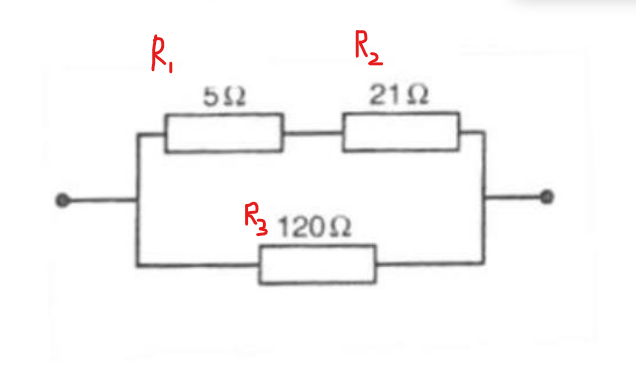
\includegraphics[width=0.5\textwidth]{figures/resistans.png}
    \caption{Indtegning af navne samt resistorkobling}
\end{figure}
Herefter skal man finde frem til værdien for den samlede erstatningsresistansen, da det er i en parallelforbindelsen anvendes formlen for en parallelforbindelse.
=======
I denne opgave skal i beregne modstanden for en parallel forbindelse som også har en serie forbindelse. I vores parallel forbindelse har vi en side der har en serie forbindelse hvor den første modstand er på 5~$\Omega$ og den anden er på 21~$\Omega$, på den anden side har vi kun 1 modstand som er på 120~$\Omega$.\newline
Før vi kan beregne den totale modstand skal vi først finde modstanden for serie forbindelsen ved brug af denne formel.
>>>>>>> 5190b2947b98483391185ccf7d0d94fa1a8cbc59
\begin{equation*}
    R_{12}=R_{1}+R_{2}
\end{equation*}
\begin{equation*}
    \mathcolorbox{yellow}{R=5\Omega+21\Omega=26\Omega}
\end{equation*}
Formlen for en parallel forbindelse ser sådan ud:
\begin{equation*}
    \frac{1}{R_{total}}=\frac{1}{R_{1}}+\frac{1}{R_{2}}
\end{equation*}
\begin{equation*}
    \frac{1}{R}=\frac{1}{26\Omega}+\frac{1}{120\Omega}=0,04679\Omega^{-1}=21,37\Omega
\end{equation*}

\subsection{Modstanden på 5~$\Omega$ laves af en kobbertråd med længden 60m. Bestem trådens radius.}
For at beregne kobbertrådens radius kan vi bruge følgende formel:
\begin{equation*}
    R=\rho\cdot\frac{l}{A}
\end{equation*}
R = Modstand i ohm (~$\Omega$)\newline
\begin{math}
    \rho = \text{Resistivitet (for kobbertråden er den på } 0.0155 \frac{\Omega \cdot mm^{2}}{m})
\end{math}\newline
l = Længden af kobbertråden\newline
A = Tværsnitsarealet\newline

For at bruge denne formel skal vi have isoleret A og derfor bliver formlen til.
\begin{equation*}
    A=\frac{l\cdot\rho}{R}
\end{equation*}
Nu kan vi indsætte vores værdier
\begin{equation*}
    A=\frac{60m\cdot0,0155\frac{\Omega\cdot mm^{2}}{m}}{5\Omega}
\end{equation*}
\begin{equation*}
    A=\frac{0,93mm^{2}}{5\Omega}=0,186mm^{2}
\end{equation*}
Nu har vi arealet af en cirkel som betyder at vi kan bruge bruge formlen for arealet af en cirkel og isolere radiussen
\begin{equation*}
    A=\pi*r^{2}
\end{equation*}
\begin{equation*}
    r^{2}=\frac{A}{\pi}
\end{equation*}
\begin{equation*}
    r=\sqrt{\frac{A}{\pi}}
\end{equation*}
\begin{equation*}
    r=\sqrt{\frac{0,186mm^{2}}{\pi}} = \sqrt{\frac{0,186}{\pi}} = 0,243mm
\end{equation*}

\subsection{Et batteri med hvilespændingen 1,4V og en indre modstand på 0,5~$\Omega$ tilsluttes resistorkoblingen. Skitser situationen og beregn polspændingen.}
\begin{equation*}
    U_{pol}=U_{hvile}-I\cdot R_{indre}
\end{equation*}
\begin{equation*}
    I_{total}=\frac{1,4V}{21,37\Omega+0,5\Omega}=0,064A
\end{equation*}

\begin{equation*}
    U_{pol}=1,4V-0,5\Omega\cdot 0,064A=1,368V
\end{equation*}
\newpage